\chapter{Auswertung und Diskussion}
\label{chap:evaluation}

Nachfolgend sollen nun die Ergebnisse der Migration der zwei Projekte Components und Helios, die mit Hilfe des umgesetzten Flow-Transpilers durchgeführt wurde, dargelegt werden. Dabei wird zum einen die Erfüllung der Zielvorgaben aus Abschnitt~\ref{sec:goals}, zum anderen die Einhaltung der technischen Anforderungen an den Transcompiler aus Abschnitt~\ref{sec:requirements} beurteilt und kritisch diskutiert. Damit die erzielten Ergebnisse besser eingeordnet werden können, werden diese hierbei auch wo möglich mit den Ansätzen von \textit{Kikura}~\autocite{KIKURA:FLOW_TO_TS} und \textit{Barabash}~\autocite{BARABASH:FLOW_TO_TS} zur Transpilierung von Flow verglichen\footnote{Vgl. Abschnitt~\ref{sec:evaluation-other-transpilers}.}. Zunächst wird jedoch die Durchführung der Migration an sich beschrieben.

\section{Durchführung der Migration}

Bereits während der Entwicklungsphase des Flow-Transpilers wurde dieser immer wieder mit dem Quelltext der vorliegenden Projekte von TeamShirts erprobt, um dessen Praxistauglichkeit anhand einer realen Codebasis zu überprüfen. Nachdem der vollständige Funktionsumfang des Transcompilers hergestellt war, wurde als erstes das Projekt Components, danach Helios mit Hilfe des Übersetzers in TypeScript umgewandelt. Diese Reihenfolge wurde bewusst gewählt, da Components keine Abhängigkeit zu anderen Projekten von TeamShirts besitzt, aber Helios wiederum Teile von Components verwendet. Weil Components somit bei der Migration von Helios bereits in TypeScript vorlag, konnte die Typisierung dieser externen Module direkt in die Typüberprüfung von Helios miteinbezogen werden.

Unmittelbar nach Ausführung des Transpilers wurden bei Components 543 und bei Helios 404 neue Typfehler durch den TypeScript-Compiler festgestellt. Diese mussten daraufhin manuell behoben werden, um die Typkorrektheit wiederherzustellen. Die Berichtigung der Typisierung vereinnahmte bei Components sieben und bei Helios acht Personentage. Aufgrund der prinzipiellen Unterschiede der Typsysteme von Flow und Typescript, die im Grundlagenteil bereits dargelegt wurden, war das Auftreten neuer Fehler zu erwarten. Wie beschrieben ist beispielsweise die Typinferenz und die Berechnung der Typkompatibilität (nominal versus strukturell) in TypeScript anders umgesetzt als bei Flow.

% Im nachfolgenden Abschnitt wird dieser Aspekt näher beleuchtet und genauer beschrieben, welche Arten von Typfehlern neu aufgetreten sind. Weiterhin wird untersucht, welche der neu erkannten Typfehler tatsächlich bislang unentdeckte Programmfehler repräsentieren.

\section{Bewertung der Ergebnisse hinsichtlich der Zielvorgabe}

Nachdem der Wechsel zu TypeScript vollzogen war konnten verschiedene Auswertungen durchgeführt werden, um die Ergebnisse bezüglich der Zielsetzung zu bewerten. Im Folgenden sollen die in Kapitel~\ref{chap:analysis} dargelegten Vorgaben hinsichtlich ihrer Erfüllung untersucht werden.

\subsection{Erkennung weiterer Typ- und Programmfehler}
\label{goal:new-type-errors}

\subsubsection{Neu aufgetretene Typfehler}

Das primäre Ziel der Migration zu TypeScript war es weitere Typ- und Programmfehler im bestehenden und zukünftigen Quelltext der Projekte von TeamShirts aufzudecken. Nach der Übersetzung der Flow-Typisierung nach TypeScript wurden sowohl in Components, als auch in Helios zahlreiche neue Typfehler festgestellt. Wie bereits ausgeführt, bietet der TypeScript-Compiler die Option \enquote{\code{strict}} um die Strenge der Typüberprüfungen deutlich zu verschärfen, indem beispielsweise die implizite Zuweisung des dynamischen Typs \code{any} verboten wird~\autocite{TSC:OPTIONS}. Tabelle~\ref{tab:type-errors} auf Seite~\pageref{tab:type-errors} gibt einen Überblick über die Anzahl und die Art der zwölf häufigsten strikten und nicht-strikten Typfehler, die unmittelbar nach der Transpilierung der zwei Projekte erkannt wurden. Insgesamt wurden bei Components 608 bzw. 543 und bei Helios 697 bzw. 404 strikte bzw. nicht-strikte Typverletzungen offen gelegt. Im Folgenden soll näher beleuchtet werden welche Arten von neuen Typfehlern überwiegend aufgedeckt wurden.

\medbreak
\begin{table}[p]
  \caption{Auflistung der zwölf häufigsten nach der Transpilierung neu aufgetretene strikten und nicht-strikten TypeScript-Typfehler in den Projekten Components und Helios.}
  \small
  \begin{tabu} to \textwidth {@{}rrrr|rrrrX@{}}
    \midrule
    \rowfont[r]{\libertineSB} Strikt & Art & Nicht-strikt & Art & Strikt & Art & Nicht-strikt & Art & {} \\
    \midrule
    249 & TS2322 & 184 & TS2322 & 205 & TS2307 & 205 & TS2307 & {} \\
    104 & TS2345 &  91 & TS2345 & 202 & TS2339 &  88 & TS2322 & {} \\
     70 & TS2339 &  70 & TS2339 & 147 & TS2322 &  37 & TS2345 & {} \\
     47 & TS2605 &  48 & TS2605 &  72 & TS2345 &  24 & TS2339 & {} \\
     39 & TS2304 &  39 & TS2304 &  24 & TS2305 &  24 & TS2305 & {} \\
     22 & TS2741 &  25 & TS2538 &  15 & TS2304 &  15 & TS2304 & {} \\
     22 & TS2554 &  23 & TS2741 &   9 & TS2531 &   3 & TS2739 & {} \\
     12 & TS2739 &  22 & TS2554 &   7 & TS2532 &   3 & TS2724 & {} \\
      9 & TS2307 &  12 & TS2739 &   4 & TS2538 &   2 & TS2605 & {} \\
      8 & TS2740 &   9 & TS2307 &   3 & TS2724 &   1 & TS2740 & {} \\
      5 & TS2557 &   5 & TS2557 &   2 & TS2739 &   1 & TS2678 & {} \\
      5 & TS2305 &   5 & TS2305 &   2 & TS2605 &   1 & TS2374 & {} \\
      4 & TS1099 &   4 & TS1099 &   1 & TS2740 &  -- & --     & {} \\
    \midrule
    \multicolumn{4}{c}{\large\textsc{components}} & \multicolumn{4}{c}{\large\textsc{helios}} & {} \\
    \midrule
  \end{tabu}
  \vspace{1.25\baselineskip}
  \caption*{
    \small
    {\libertineSB{Arten von Typfehlern}~\autocite{TYPESCRIPT:GITHUB}}\\
    \vspace{.5\baselineskip}
    TS1099 -- Die Liste der Typargumente darf nicht leer sein.\\
    TS2304 -- Name $x$ kann nicht gefunden werden.\\
    TS2305 -- Modul $x$ exportiert kein Element $y$.\\
    TS2307 -- Modul $x$ kann nicht gefunden werden.\\
    TS2322 -- Typ $x$ ist Typ $y$ nicht zuweisbar.\\
    TS2339 -- Attribut $x$ existiert nicht in Typ $y$.\\
    TS2345 -- Argument mit Typ $x$ ist Parameter mit Typ $y$ nicht zuweisbar.\\
    TS2374 -- Doppelte Index-Signatur für Zeichenketten.\\
    TS2531 -- Objekt ist möglicherweise \code{null}.\\
    TS2532 -- Objekt ist möglicherweise \code{undefined}.\\
    TS2538 -- Typ $x$ darf nicht als Index-Typ verwendet werden.\\
    TS2554 -- $x$ Argumente erwartet, aber $y$ gegeben (Anzahl).\\
    TS2557 -- Mindestens $x$ Argumente erwartet, aber $y$ oder mehr gegeben (Anzahl).\\
    TS2605 -- Der Typ des JSX-Elements $x$ ist keine Konstruktorfunktion eines JSX-Elements.\\
    TS2678 -- Typ $x$ ist nicht vergleichbar mit Typ $y$.\\
    TS2724 -- Modul $x$ exportiert kein Element $y$. Meinten Sie $z$?\\
    TS2739 -- Typ $x$ fehlen die folgenden Attribute von Typ $y$: $z$.\\
    TS2740 -- Typ $x$ fehlen die folgenden Attribute von Typ $y$: $z$ und weiterhin $p$.\\
    TS2741 -- Attribut $x$ fehlt in Typ $y$, wird aber von Typ $z$ erwartet.\\
  }
  \vspace{\baselineskip}
  \label{tab:type-errors}
\end{table}


Bei beiden Projekten treten am häufigsten Typfehler auf, die sich darauf beziehen, dass Typen einander nicht zuweisbar sind oder dass Typen ein referenziertes Attribut nicht beinhalten (TS2322, TS2345 bzw. TS2339). Die Gründe für diese Fehler sind vielfältig: Wie dargelegt unterscheiden sich Flow und TypeScript in einigen Aspekten wie der Typinferenz und der Betrachtung von Subtypen grundlegend, sodass hierdurch neue Typverletzungen entstehen können. Darüber hinaus wurden nach Ausführung des Transpilers externe Typdefinitionen für die eingesetzten Bibliotheken hinzugefügt, um deren korrekte Verwendung zu überprüfen. Weil die bestehende Typisierung von Ausdrücken nicht überall mit diesen Typdeklarationen übereinstimmt, bilden sich auch so neue Typfehler. Bei Helios tritt die Typverletzung TS2307, also dass ein Modul nicht gefunden werden kann, am öftesten auf. Dieser Fehler resultiert daraus, dass in diesem Projekt neben regulären TypeScript-Modulen auch andere Dateitypen wie beispielsweise SVG-Dateien importiert werden, was bei TypeScript normalerweise nicht möglich ist. Um eine derartige Verarbeitung weiterer Dateitypen zu realisieren, wird spezielle Software wie \textit{Webpack}~\autocite{WEBPACK} eingesetzt, die eine solche Modulstruktur zu statischen Ausgabedateien transformiert. Durch Anlegen einer globalen Typdeklaration für \enquote{Module} derartiger Dateitypen kann diese Klasse von Typfehlern aber leicht behoben werden (vgl. Quelltext~\ref{code:fix-webpack-imports}). Ein weiterer häufiger Fehler ist, dass der Import von Typen aus Bibliotheken fehlschlägt, wenn sich zum Beispiel deren Name in TypeScript geändert hat (TS2305). Außerdem entstehen Typfehler, wenn in Flow globale Typen der Standardbibliothek eingesetzt werden, da diese in TypeScript vor deren Verwendung erst explizit importiert werden müssen (TS2304). Idealerweise sollte der Import dieser zuvor globalen Typen durch den Transpiler, ähnlich zu der in Abschnitt~\ref{sec:react-type-import-mapping} beschriebenen Übersetzung der React-Typimporte, automatisch durchgeführt werden, um den Aufwand manueller Korrekturen nach der Transpilierung zu reduzieren. Eine weitere Art von Fehler, die vor allem bei Components vermehrt auftritt, betrifft die inkorrekte Typisierung von React"=Komponenten~(TS2605).

\begin{lstlisting}[
  float,
  floatplacement=H,
  label={code:fix-webpack-imports},
  caption={Behebung des Fehlers TS2307 durch globale Deklarationen von SVG-Modulen.},
]
declare module '*.svg' {
  export default SVGElement;
}
\end{lstlisting}

\subsubsection{Neu erkannte Programmfehler}

Ein Aspekt der Zielsetzung war auch fehlerhaftes Programmverhalten aufzudecken. Während der manuellen Behebung der neu aufgetreten Typverletzungen wurde deshalb untersucht, ob manche der Typfehler tatsächlich semantische Probleme innerhalb des Quelltexts repräsentieren. In der Tat konnten einige Programmfehler durch TypeScript ermittelt werden. Anhand von drei Beispielen soll im Folgenden dargelegt werden, welche Art von Programmfehlern dabei festgestellt wurden. Obwohl keiner der Fälle kritische Laufzeitfehler verursacht, ist es dennoch erstrebenswert diese zu korrigieren, um die Codequalität insgesamt zu steigern.

\vspace{-0.5\baselineskip}
\paragraph{Zusätzliche Objektattribute bei Funktionsargumenten}
Ein Beispiel für derartige Programmfehler ist der inkorrekte Aufruf von Funktionen, die ein Objekt mit verschiedenen Attributen als Argument erwarten. Weil Flow es standardmäßig erlaubt, dass bei Objektliteralen Attribute angegeben werden, die nicht durch den zugrunde liegende Objekttyp spezifiziert sind~\autocite{FLOW:WIDTH_SUBTYPING}, ist der Fehler bislang unerkannt geblieben. TypeScript behandelt Objekttypen dagegen wie ausgeführt immer exakt, sodass zusätzliche Attribute eine Typverletzung darstellen und der fehlerhafte Funktionsaufruf damit aufgedeckt wird.

\vspace{-0.5\baselineskip}
\paragraph{Fehlerhafte Verwendung von React-Komponenten}
React-Komponenten werden ähnlich wie HTML-Elemente eingesetzt und sind in der Regel durch JSX-Syntax aufgebaut. Mittels selbstdefinierter Attribute können dabei verschiedene Eigenschaften der Komponente festgelegt werden. In einigen Fällen wurde von TypeScript erkannt, dass bei Komponenten Attribute angegeben wurden, die nicht länger bestehen. Weil React-Komponenten intern durch Objekte implementiert werden, die deren Struktur und Attribute beschreiben~\autocite{REACT:REACT_ELEMENTS}, kann die gleiche Argumentation wie zuvor als Grund für die unterschiedliche Ergebnisse bei Flow und TypeScript herangezogenen werden: Da TypeScript im Gegensatz zu Flow alle Objekte stets exakt betrachtet, stellen zusätzliche angegebene Attribute bei Komponenten eine Typverletzung dar.

\vspace{-0.5\baselineskip}
\paragraph{Falscher Argumenttyp bei Funktionsaufrufen}
Zuletzt wurde festgestellt, dass der Typ mancher Funktionsargumente nicht mit dem erwarteten Typ übereinstimmt. Weil die Argumente im aufgetretenen Fall unmittelbar vor Weitergabe an die Funktion durch eine weitere Bibliotheksfunktion umgeformt werden und für diese zweite Funktion in Flow keine Typisierung vorliegt, wurde der Rückgabetyp hier implizit zu \code{any} umgeformt. Weil \code{any} jedem Typ zuweisbar ist, wurden die Rückgabewerte der Bibliotheksfunktion als Argument der ersten Funktion akzeptiert, obwohl die Typen in Wahrheit inkompatibel sind. Der Aufruf schläg zur Laufzeit nur deshalb nicht fehl, weil der Typ des Rückgabewert mittels der dynamischen Typumwandlung von JavaScript implizit angepasst wird. In TypeScript wird dieser Typfehler statisch erkannt, da für die beteiligte Bibliothek eine externe Typdefinition hinzugefügt wurde, sodass die Inkompatibilität der Typen aufgedeckt wird.

\subsubsection{Fazit}

Es gilt hervorzuheben, dass die Typfehler nach der Migration größtenteils keine Programmfehler darstellen, sondern entweder auf die grundlegenden Unterschiede von Flow und TypeScript oder auf Unzulänglichkeiten der vorherigen Typisierung durch Flow zurückzuführen sind. Auch die Integration externer Typdefinitionen für die eingesetzten Bibliotheken steigerte zwar die Abdeckung der Projekte durch das Typsystem, aber gleichzeitig wurden hierdurch neue Typfehler eingeführt. Dass mit dem Wechsel zu TypeScript eine hohe Zahl zuvor unerkannter kritischer Laufzeitfehler in den Projekten gefunden wird, war aufgrund der kontinuierlichen maschinellen und menschlichen Softwaretests unwahrscheinlich, da angenommen werden kann, dass fatale Fehler im Allgemeinen ohnehin bereits im Vorfeld entdeckt worden wären. Wie dargelegt konnten durch den Wechsel zu TypeScript aber dennoch einerseits einige tatsächliche unkritische Programmfehler aufgedeckt werden, andererseits allgemeine Schwächen der bisherigen Typisierung offen gelegt werden. Deshalb kann die Zielsetzung insgesamt als erfüllt betrachtet werden.

\subsection{Unterstützung externer Bibliotheken}

Die Migration zu TypeScript wurde weiterhin angestrebt, weil vermutet wird, dass hier Typdeklarationen für eine insgesamt größere Zahl von JavaScript-Bibliotheken vorliegen und diese aktueller sind als bei Flow. Im Folgenden soll beleuchtet werden, ob dies tatsächlich zutrifft. Wie ausgeführt stellen einige Projekte selbst Definitionsdateien mit der Typisierung bereit, bei anderen kann auf separat gepflegte Typisierungen zurückgegriffen werden

Für Flow und TypeScript existiert jeweils ein Projekt mit dem Ziel Typdeklarationen für die gängigsten JavaScript-Bibliotheken bereitzustellen. Während seit 2012 für TypeScript das Projekt \textit{DefinitelyTyped}~\autocite{DEFINITELY_TYPED} besteht, ist 2017 für Flow ein vergleichbarer Ansatz namens \textit{flow-typed}~\autocite{FLOW_TYPED} entstanden. Im Allgemeinen kann angenommen werden, dass Bibliotheken, die ihre eigenen Typdeklarationen mitliefern, aktueller und korrekter sind, weil im Zuge der Veröffentlichung neuer Versionen in der Regel auch die Typisierung durch den Autor entsprechend aktualisiert wird\footnote{Im Falle von TypeScript können die Definitionsdateien beispielsweise auch durch den TypeScript-Compiler automatisch erzeugt werden~\autocite{TSC:OPTIONS}.}. Bei der nachträglichen Erstellung von Typdeklarationen durch die Entwickler-Gemeinschaft besteht die Gefahr, dass die Typisierung das Verhalten der Bibliothek nicht richtig abbildet oder dass diese veralten. Deshalb sind Typdefinitionen, die von den Projekten selbst verwaltet werden, generell zu bevorzugen. Zunächst sollen \textit{DefinitelyTyped} und \textit{flow-typed} in Tabelle~\ref{tab:libdefs} mittels verschiedener Kennzahlen allgemein verglichen werden, um die Verfügbarkeit von gemeinschaftlich gepflegten Typdeklarationen zu untersuchen. Wie die Zahl der Git-Commits und der Beitragenden im Jahresmittel belegt, weist \textit{DefinitelyTyped} eine deutlich größere Aktivität als \textit{flow-typed} auf. Insgesamt werden bei TypeScript in etwa zehn mal mehr Bibliotheken unterstützt, als bei Flow, was trotz des Umstands, dass \textit{DefinitelyTyped} fünf Jahre älter ist, einen beachtlichen Faktor darstellt.

\medbreak
\begin{table}[tbh]
  \caption{Verschiedene Eigenschaften der Projekte \textit{DefinitelyTyped} und \textit{flow-typed} auf der Software-Plattform GitHub~\autocite{GITHUB} (Stand: Oktober 2019).}
  \footnotesize
  \begin{tabu} to \textwidth {@{}lrrrrX@{}}
    \midrule
    \rowfont[l]{\libertineSB} Projekt & Typdefinitionen & Commits & Beitragende & Sterne & {} \\
    \midrule
    flow-typed      &  628 &  2.600~~~~~520 p.~a. &   800~~~~~201  p.~a. &  3.400 & {} \\
    DefinitelyTyped & 6202 & 65.500~~~8188 p.~a. & 9.800~~~1785  p.~a. & 25.000 & {} \\
    \midrule
  \end{tabu}
  \vspace{0.75\baselineskip}
  \caption*{
    \footnotesize
    Quelle der Aktivitätsdaten: Analyse der Git-Repositories mit \textit{GitStats}~\autocite{GITSTATS}.\\
    Angaben pro Jahr (p.~a.) stellen den Durchschnitt aller Jahre dar.
  }
  \label{tab:libdefs}
\end{table}


Nachfolgend wird nun die Unterstützung externer Bibliotheken anhand der 15 am häufigsten eingesetzten Pakete innerhalb der zwei Projekte von TeamShirts in Tabelle~\ref{tab:used-libraries} konkret betrachtet. Die Bibliotheken, die am öftesten verwendet werden, wurden durch statische Analyse des Quelltexts ermittelt, indem gezählt wurde, wie oft diese jeweils importiert werden. Für diese Auswahl wurde anschließend untersucht, ob einerseits für Flow und TypeScript generell Typdeklarationen bestehen, andererseits in welcher Form diese gegebenenfalls vorliegen (als Bestandteil der Bibliothek oder separat erstellt). Weiterhin wurde beleuchtet, ob die Typdefinitionen der aktuellen Version des Pakets entsprechen oder veraltet sind. Dabei wird nur die Haupt- und Nebenversionsnummer\footnote{Vgl. \textit{Semantic Versioning}~\autocite{SEMANTIC_VERSIONING}.} der Pakete betrachtet, weil die Revisionsnummer nur der Behebung von Programmfehlern dient und per Definition die Schnittstellen nicht verändern darf. Bei \textit{flow-typed} wird die Kompatibilität der Typdefinitionen allerdings nur für die Hauptversion angegeben, sodass unklar ist, inwieweit die Deklarationen tatsächlich alle Funktionen der aktuellen Nebenversion abbilden. \textit{DefinitelyTyped} differenziert hier stärker und gibt jeweils für alle Pakete exakte Versionsnummern an, wodurch die Aktualität besser eingeschätzt werden kann.

\medbreak
\begin{table}[tbh]
  \caption{Verfügbarkeit von Typdeklarationen für Flow beziehungsweise TypeScript für die 15 am häufigsten verwendeten JavaScript"=Bibliotheken innerhalb der Projekte Components und Helios.}
  \footnotesize
  \begin{tabu} to \textwidth {@{}CrrrrX@{}}
    \midrule
    \rowfont[l]{\libertineSB} Bibliothek & Version & Verwendung & Verfügb. Flow & Verfügb. TypeScript & {} \\
    \midrule
    react             & 16.11 &	388 & 16.11~~~~~~\code{I}  & 16.11~~~~~~\code{E} & {} \\
    styled-components &   4.4 &	135 &   4.x~~~~~~\code{E}  &   4.1~~~~~~\code{E} & {} \\
    @storybook/react  &   5.2 &  74 &   5.x~~~~~~\code{E}  &   4.0~~~~~~\code{E} & {} \\
    chai              &   4.2 &  73 &   4.x~~~~~~\code{E}  &   4.2~~~~~~\code{E} & {} \\
    react-redux       &   7.1 &	 72 &   7.x~~~~~~\code{E}  &   7.1~~~~~~\code{E} & {} \\
    react-apollo      &   3.1 &  34 &    --~~~~~~\code{ }  &   3.1~~~~~~\code{I} & {} \\
    react-router-dom  &   5.1 &  22 &   5.x~~~~~~\code{E}  &   5.1~~~~~~\code{E} & {} \\
    react-loadable    &   5.5 &  17 &   5.x~~~~~~\code{E}  &   5.5~~~~~~\code{E} & {} \\
    lodash            &  4.17 &  15 &   4.x~~~~~~\code{E}  &  4.14~~~~~~\code{E} & {} \\
    react-router      &   5.1 &  13 &   5.x~~~~~~\code{E}  &   5.1~~~~~~\code{E} & {} \\
    es6-error         &   4.1 &   9 &   4.x~~~~~~\code{E}  &   4.1~~~~~~\code{I} & {} \\
    react-motion      &   0.5 &   5 &    --~~~~~~\code{ }  &  0.29~~~~~~\code{E} & {} \\
    axios             &  0.19 &   3 &  0.19~~~~~~\code{E}  &  0.19~~~~~~\code{I} & {} \\
    react-collapse    &   5.0 &   3 &    --~~~~~~\code{ }  &   4.0~~~~~~\code{E} & {} \\
    css-math          &   0.4 &   2 &    --~~~~~~\code{ }  &    --~~~~~~\code{ } & {} \\
    \midrule
  \end{tabu}
  \vspace{0.75\baselineskip}
  \caption*{
    \footnotesize
    \code{E}: Separat gepflegte Typdefinition (durch \textit{flow-typed} beziehungsweise \textit{DefinitelyTyped})\\
    \code{I}: In Bibliothek integrierte Typdefinition
  }
  \label{tab:used-libraries}
\end{table}


Während bei Flow für vier der 15 Bibliotheken keine Typdefinition vorliegt, existiert bei TypeScript lediglich in einem Fall keine Typisierung. Der Großteil der Deklarationen entstammt jeweils den Projekten \textit{flow-typed} bzw. \textit{DefinitelyTyped}. Nur in einem bzw. drei Fällen bei Flow bzw. TypeScript sind die Typdefinitionen direkt in die Pakete integriert.
Für den Großteil der Bibliotheken sind die Typisierungen sowohl bei Flow, als auch bei TypeScript aktuell. Nur bei TypeScript besteht in zwei bzw. drei Fällen eine Abweichung von der Haupt- bzw. Nebenversion. Aus den dargelegten Gründen kann nicht überprüft werden, ob auch bei Flow veraltete Typdefinitionen hinsichtlich der Nebenversion vorliegen, weil diese durch \textit{flow-typed} nicht angegeben wird. Da bei TypeScript für die gegebenen Projekte von TeamShirts eine größere Zahl von Bibliotheken durch Typdeklarationen abgebildet werden und diese in höherem Maße in die Pakete integriert sind, kann die Zielsetzung, externe Bibliotheken besser zu unterstützen, insgesamt als erreicht betrachtet werden. Kritisch anzumerken ist aber, dass bei TypeScript für fünf Bibliotheken keine vollständig aktuelle Version vorliegt. Jedoch ist dies auch bei Flow nicht gesichert.

\subsection{Performance der Typüberprüfungen}

\subsubsection{Messung der Laufzeit der Typüberprüfungen}

Eine weitere Zielsetzung des Wechsels zu TypeScript war die Performance der Typüberprüfungen zu verbessern, das heißt deren Laufzeit zu verringern. Nachdem die Migration der zwei Projekte abgeschlossen war, konnten die Laufzeiten der vollständigen Typüberprüfung durch Flow bzw. TypeScript ermittelt werden. Auch die Messung der Zeitspanne von inkrementellen Überprüfungen durch den Flow- bzw. TypeScript-Sprachserver wurde durch Auswertung der Logdateien angestrebt. Jedoch ist dieser Ansatz nur möglich, wenn ein Editor ausgeführt wird, der den jeweiligen Server startet und daraufhin Anfragen bezüglich der Typisierung an diesen stellt. Weil die Ergebnisse somit stark von der Implementierung des Editors abhängen, besteht die Gefahr, dass diese verfälscht werden und wenig aussagekräftig sind. Deshalb werden inkrementelle Typüberprüfungen nachfolgend nicht betrachtet.

Zur Bestimmung der Laufzeit der vollständigen Berechnung wurden in beiden Projekten für Flow und TypeScript jeweils 100 Proben (\textit{Samples}) mit Hilfe des GNU-Programms \textit{time}~\autocite{GNU_TIME} gemessen und die zehn kleinsten und größten Werte daraufhin verworfen, um den Einfluss von \enquote{Ausreißern} zu minimieren. Aus den verbleibenden 80 Werten wurde anschließend der Mittelwert gebildet und die Standardabweichung berechnet. Dabei wurde in allen Messungen die zum damaligen Zeitpunkt aktuelle Version~3.5 von TypeScript und die von TeamShirts eingesetzte Version~0.96 von Flow verwendet. Um auch den Einfluss von unterschiedlich leistungsfähiger Hardware miteinzubeziehen, wurden die Messreihen auf vier verschiedenen Systemen durchgeführt:

\begin{enumerate}[label=\Alph*.]
  \item AMD Phenom II X6 1055T Prozessor mit 2,9~GHz\footnote{Es wird jeweils der Grundtakt des Prozessors und nicht der maximal mögliche Wert durch dynamische Übertaktung angegeben.} und 6 Rechenkernen (2010)\\16~GB Arbeitsspeicher, Solid State Drive, Arch Linux
  \item Intel Core i5-4258U Prozessor mit 2,4~GHz und 4 Rechenkernen (2013)\\8~GB Arbeitsspeicher, Solid State Drive, Arch Linux
  \item Intel Core i5-4210M Prozessor mit 2,6~GHz und 4 Rechenkernen (2014)\\16~GB Arbeitsspeicher, Solid State Drive, Arch Linux
  \item Intel Core i7-6700 Prozessor mit 3,4~GHz und 8 Rechenkernen (2015)\\32~GB Arbeitsspeicher, Solid State Drive, Debian Linux
\end{enumerate}

Die durch diese Methodik ermittelten Messwerte, deren Standardabweichung und die relative Veränderung der Laufzeiten werden in Tabelle~\ref{tab:performance-complete} für beide Projekte aufgelistet: Offensichtlich beschleunigen modernere, performante Prozessoren mit höherer Taktfrequenz und größeren Caches generell die Typüberprüfung durch Flow bzw. TypeScript. Die These, dass TypeScript schneller als Flow sei, lässt sich aber nur anhand des Projekts Helios für die Systeme B, C und D belegen (vgl. negative Werte für relative Veränderung der Laufzeit). Bei Components ist TypeScript dagegen stets deutlich langsamer als Flow.

\medbreak
\begingroup
\setlength{\tabcolsep}{7pt}
\begin{table}[tbh]
  \small
  \begin{tabu} to \textwidth {@{}rrrrrr|rrrrrX@{}}
    \midrule
    {} & \multicolumn{2}{l}{\libertineSB{Flow}} & \multicolumn{2}{l}{\libertineSB{TypeScript}} & {} & \multicolumn{2}{l}{\libertineSB{Flow}} & \multicolumn{2}{l}{\libertineSB{TypeScript}} & {}\\
    \rowfont[c]{} \libertineSB{S} & Laufzeit & s & Laufzeit & s & rel. $\Delta$ & Laufzeit & s & Laufzeit & s & rel. $\Delta$ & {}\\
    \midrule
    A & 7,87 & 0,09 & 15,50 & 0,08 & 97,0\% & 12,20 & 0,16 & 13,06 & 0,70 &   7,1\% & {} \\
    B & 6,86 & 0,05 & 10,59 & 0,06 & 54,4\% & 10,90 & 0,33 &  8,49 & 0,16 & -22,1\% & {} \\
    C & 6,50 & 0,02 &  9,56 & 0,05 & 47,1\% & 11,70 & 0,07 &  7,63 & 0,04 & -34,8\% & {} \\
    D & 3,38 & 0,02 &  6,41 & 0,04 & 89,6\% &  5,15 & 0,02 &  4,94 & 0,03 &  -4,1\% & {} \\
    \midrule
    {} & \multicolumn{5}{c}{\large\textsc{components}} & \multicolumn{5}{c}{\large\textsc{helios}} & {}\\
    \midrule
  \end{tabu}
  \caption{Durchschnittliche Laufzeit in Sekunden, Standardabweichung (s) und relative Veränderung der Zeitspanne (rel. $\Delta$) der vollständigen Typüberprüfung der Projekte Components und Helios durch Flow 0.96 und TypeScript 3.5 auf verschiedenen Hardware-Systemen (S).}
  \label{tab:performance-complete}
\end{table}
\endgroup


Wie im Grundlagenteil bereits ausgeführt, wird die Berechnung der Typkorrektheit durch Flow stark parallelisiert, um deren Laufzeit zu verringern. TypeScript bietet keine Unterstützung für eine nebenläufige Typüberprüfung durch mehrere Threads~\autocite{TS:NO_MULTICORE}, sodass die Performance hier vorrangig von der Leistungsfähigkeit der einzelnen Prozessorkerne abzuhängen scheint. Diese These wird durch die gemessenen Daten unterstützt, denn je performanter die Rechenkerne sind, desto kleiner wird die Differenz zwischen den Laufzeiten von Flow und TypeScript bei Components bzw. desto größer wird diese bei Helios.
Für System D scheint jedoch die Parallelisierung von Flow aufgrund der hohen Zahl von acht Prozessorkernen den größeren Einfluss zu nehmen, als die Leistungsfähigkeit der einzelnen Kerne. Weil die Systeme B und C jeweils nur über vier Rechenkerne verfügen, ist der Effekt der Nebenläufigkeit hier kleiner. Als einen möglichen Grund, warum Components im Vergleich zu Helios durch Flow insgesamt schneller überprüft werden kann, kann angeführt werden, dass dieses Projekt aus einer Vielzahl unabhängiger Komponenten besteht deren Verarbeitung somit gut durch Flow parallelisiert werden kann. In Helios besteht eine größere Abhängigkeit der Module untereinander.

\subsubsection{Einfluss von Parallelisierung auf die Laufzeiten}

Der Einfluss der Parallelisierung auf die Laufzeit der Berechnungen soll im Folgenden näher beleuchtet werden. Hierfür wurde eine weitere Testreihe durchgeführt in welcher die Zahl der einsetzbaren Rechenkerne für die Berechnung durch das Linux-Programm \textit{taskset}~\autocite{TASKSET} eingeschränkt wird. Dabei wird dem Prozess durch den Scheduler des Betriebssystems zunächst lediglich ein Rechenkern, dann zwei usw. zugeordnet. Abbildung~\ref{fig:plot-cores} auf Seite~\pageref{fig:plot-cores} zeigt jeweils ein Diagramm für Components und Helios, welches die Beeinflussung des Laufzeitverhaltens durch diese Einschränkung grafisch darstellt. Die exakten Messwerte, deren Standardabweichung und die relative Veränderung wird darüber hinaus in Tabelle~\ref{tab:performance-cores} aufgelistet.

\medbreak
\begingroup
\setlength{\tabcolsep}{7pt}
\begin{table}[tbh]
  \caption[Durchschnittliche Laufzeit in Sekunden, Standardabweichung (s) und relative Veränderung der Zeitspanne (rel. $\Delta$) der vollständigen Typüberprüfung der Projekte Components und Helios durch Flow 0.96 und TypeScript 3.5 bei zunehmender Zahl verfügbarer Rechenkerne~(K).]{Durchschnittliche Laufzeit in Sekunden, Standardabweichung (s) und relative Veränderung der Zeitspanne (rel. $\Delta$) der vollständigen Typüberprüfung der Projekte Components und Helios durch Flow 0.96 und TypeScript 3.5 bei zunehmender Zahl verfügbarer Rechen"=kerne~(K). Gemessen mit Intel Core i7-6700 CPU mit 3,4 GHz (System D).}
  \small
  \begin{tabu} to \textwidth {@{}rrrrrr|rrrrrX@{}}
    \midrule
    {} & \multicolumn{2}{l}{\libertineSB{Flow}} & \multicolumn{2}{l}{\libertineSB{TypeScript}} & {} & \multicolumn{2}{l}{\libertineSB{Flow}} & \multicolumn{2}{l}{\libertineSB{TypeScript}} & {}\\
    \rowfont[c]{} \libertineSB{K} & Laufzeit & s & Laufzeit & s & rel. $\Delta$ & Laufzeit & s & Laufzeit & s & rel. $\Delta$ & {}\\
    \midrule
    1 & 10,59 & 0,03 & 10,13 & 0,03 & -4,3\% & 17,26 & 0,05 & 8,81 & 0,01 & -49,0\% & {} \\
    2 &  6,19 & 0,02 &  6,85 & 0,05 & 10,7\% &  9,61 & 0,04 & 5,44 & 0,04 & -43,4\% & {} \\
    3 &  4,74 & 0,03 &  6,50 & 0,02 & 37,1\% &  7,23 & 0,03 & 5,03 & 0,02 & -30,4\% & {} \\
    4 &  4,05 & 0,03 &  6,43 & 0,02 & 58,8\% &  6,16 & 0,04 & 4,95 & 0,01 & -19,6\% & {} \\
    5 &  3,79 & 0,04 &  6,48 & 0,02 & 71,0\% &  5,82 & 0,03 & 5,04 & 0,15 & -13,4\% & {} \\
    6 &  3,63 & 0,02 &  6,41 & 0,04 & 76,6\% &  5,51 & 0,03 & 4,94 & 0,03 & -10,3\% & {} \\
    7 &  3,52 & 0,02 &  6,40 & 0,03 & 81,8\% &  5,31 & 0,03 & 4,93 & 0,03 &  -7,2\% & {} \\
    8 &  3,42 & 0,02 &  6,40 & 0,03 & 87,1\% &  5,16 & 0,02 & 4,94 & 0,03 &  -4,3\% & {} \\
    \midrule
    {} & \multicolumn{5}{c}{\large\textsc{components}} & \multicolumn{5}{c}{\large\textsc{helios}} & {}\\
    \midrule
  \end{tabu}
  \label{tab:performance-cores}
\end{table}
\endgroup


\begin{figure}[p]
  \centering

  % GNUPLOT: LaTeX picture with Postscript
\begingroup
  \makeatletter
  \providecommand\color[2][]{%
    \GenericError{(gnuplot) \space\space\space\@spaces}{%
      Package color not loaded in conjunction with
      terminal option `colourtext'%
    }{See the gnuplot documentation for explanation.%
    }{Either use 'blacktext' in gnuplot or load the package
      color.sty in LaTeX.}%
    \renewcommand\color[2][]{}%
  }%
  \providecommand\includegraphics[2][]{%
    \GenericError{(gnuplot) \space\space\space\@spaces}{%
      Package graphicx or graphics not loaded%
    }{See the gnuplot documentation for explanation.%
    }{The gnuplot epslatex terminal needs graphicx.sty or graphics.sty.}%
    \renewcommand\includegraphics[2][]{}%
  }%
  \providecommand\rotatebox[2]{#2}%
  \@ifundefined{ifGPcolor}{%
    \newif\ifGPcolor
    \GPcolortrue
  }{}%
  \@ifundefined{ifGPblacktext}{%
    \newif\ifGPblacktext
    \GPblacktexttrue
  }{}%
  % define a \g@addto@macro without @ in the name:
  \let\gplgaddtomacro\g@addto@macro
  % define empty templates for all commands taking text:
  \gdef\gplbacktext{}%
  \gdef\gplfronttext{}%
  \makeatother
  \ifGPblacktext
    % no textcolor at all
    \def\colorrgb#1{}%
    \def\colorgray#1{}%
  \else
    % gray or color?
    \ifGPcolor
      \def\colorrgb#1{\color[rgb]{#1}}%
      \def\colorgray#1{\color[gray]{#1}}%
      \expandafter\def\csname LTw\endcsname{\color{white}}%
      \expandafter\def\csname LTb\endcsname{\color{black}}%
      \expandafter\def\csname LTa\endcsname{\color{black}}%
      \expandafter\def\csname LT0\endcsname{\color[rgb]{1,0,0}}%
      \expandafter\def\csname LT1\endcsname{\color[rgb]{0,1,0}}%
      \expandafter\def\csname LT2\endcsname{\color[rgb]{0,0,1}}%
      \expandafter\def\csname LT3\endcsname{\color[rgb]{1,0,1}}%
      \expandafter\def\csname LT4\endcsname{\color[rgb]{0,1,1}}%
      \expandafter\def\csname LT5\endcsname{\color[rgb]{1,1,0}}%
      \expandafter\def\csname LT6\endcsname{\color[rgb]{0,0,0}}%
      \expandafter\def\csname LT7\endcsname{\color[rgb]{1,0.3,0}}%
      \expandafter\def\csname LT8\endcsname{\color[rgb]{0.5,0.5,0.5}}%
    \else
      % gray
      \def\colorrgb#1{\color{black}}%
      \def\colorgray#1{\color[gray]{#1}}%
      \expandafter\def\csname LTw\endcsname{\color{white}}%
      \expandafter\def\csname LTb\endcsname{\color{black}}%
      \expandafter\def\csname LTa\endcsname{\color{black}}%
      \expandafter\def\csname LT0\endcsname{\color{black}}%
      \expandafter\def\csname LT1\endcsname{\color{black}}%
      \expandafter\def\csname LT2\endcsname{\color{black}}%
      \expandafter\def\csname LT3\endcsname{\color{black}}%
      \expandafter\def\csname LT4\endcsname{\color{black}}%
      \expandafter\def\csname LT5\endcsname{\color{black}}%
      \expandafter\def\csname LT6\endcsname{\color{black}}%
      \expandafter\def\csname LT7\endcsname{\color{black}}%
      \expandafter\def\csname LT8\endcsname{\color{black}}%
    \fi
  \fi
    \setlength{\unitlength}{0.0500bp}%
    \ifx\gptboxheight\undefined%
      \newlength{\gptboxheight}%
      \newlength{\gptboxwidth}%
      \newsavebox{\gptboxtext}%
    \fi%
    \setlength{\fboxrule}{0.5pt}%
    \setlength{\fboxsep}{1pt}%
\begin{picture}(7360.00,4520.00)%
    \gplgaddtomacro\gplbacktext{%
      \csname LTb\endcsname%%
      \put(596,652){\makebox(0,0)[r]{\strut{}$3$}}%
      \csname LTb\endcsname%%
      \put(596,1107){\makebox(0,0)[r]{\strut{}$4$}}%
      \csname LTb\endcsname%%
      \put(596,1563){\makebox(0,0)[r]{\strut{}$5$}}%
      \csname LTb\endcsname%%
      \put(596,2018){\makebox(0,0)[r]{\strut{}$6$}}%
      \csname LTb\endcsname%%
      \put(596,2474){\makebox(0,0)[r]{\strut{}$7$}}%
      \csname LTb\endcsname%%
      \put(596,2929){\makebox(0,0)[r]{\strut{}$8$}}%
      \csname LTb\endcsname%%
      \put(596,3384){\makebox(0,0)[r]{\strut{}$9$}}%
      \csname LTb\endcsname%%
      \put(596,3840){\makebox(0,0)[r]{\strut{}$10$}}%
      \csname LTb\endcsname%%
      \put(596,4295){\makebox(0,0)[r]{\strut{}$11$}}%
      \csname LTb\endcsname%%
      \put(1410,448){\makebox(0,0){\strut{}1}}%
      \csname LTb\endcsname%%
      \put(2111,448){\makebox(0,0){\strut{}2}}%
      \csname LTb\endcsname%%
      \put(2813,448){\makebox(0,0){\strut{}3}}%
      \csname LTb\endcsname%%
      \put(3515,448){\makebox(0,0){\strut{}4}}%
      \csname LTb\endcsname%%
      \put(4216,448){\makebox(0,0){\strut{}5}}%
      \csname LTb\endcsname%%
      \put(4918,448){\makebox(0,0){\strut{}6}}%
      \csname LTb\endcsname%%
      \put(5620,448){\makebox(0,0){\strut{}7}}%
      \csname LTb\endcsname%%
      \put(6321,448){\makebox(0,0){\strut{}8}}%
    }%
    \gplgaddtomacro\gplfronttext{%
      \csname LTb\endcsname%%
      \put(158,2473){\rotatebox{-270}{\makebox(0,0){\strut{}\small durchschnittliche Laufzeit in s}}}%
      \csname LTb\endcsname%%
      \put(3865,142){\makebox(0,0){\strut{}\small Anzahl eingesetzter Prozessorkerne}}%
      \csname LTb\endcsname%%
      \put(3865,3989){\makebox(0,0){\strut{}\small\bfseries Components}}%
      \csname LTb\endcsname%%
      \put(6158,4010){\makebox(0,0)[r]{\strut{}\small Flow}}%
      \csname LTb\endcsname%%
      \put(6158,3806){\makebox(0,0)[r]{\strut{}\small TypeScript}}%
    }%
    \gplbacktext
    \put(0,0){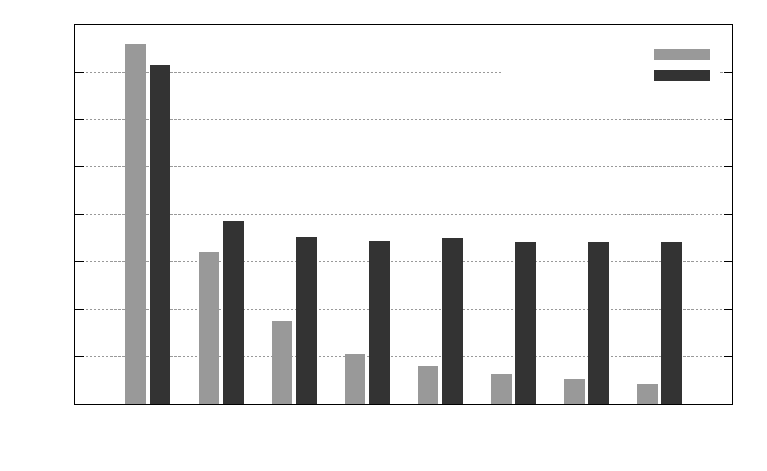
\includegraphics{../data/performance/plots/cores/components-plot}}%
    \gplfronttext
  \end{picture}%
\endgroup


  \vspace{.5\baselineskip}

  % GNUPLOT: LaTeX picture with Postscript
\begingroup
  \makeatletter
  \providecommand\color[2][]{%
    \GenericError{(gnuplot) \space\space\space\@spaces}{%
      Package color not loaded in conjunction with
      terminal option `colourtext'%
    }{See the gnuplot documentation for explanation.%
    }{Either use 'blacktext' in gnuplot or load the package
      color.sty in LaTeX.}%
    \renewcommand\color[2][]{}%
  }%
  \providecommand\includegraphics[2][]{%
    \GenericError{(gnuplot) \space\space\space\@spaces}{%
      Package graphicx or graphics not loaded%
    }{See the gnuplot documentation for explanation.%
    }{The gnuplot epslatex terminal needs graphicx.sty or graphics.sty.}%
    \renewcommand\includegraphics[2][]{}%
  }%
  \providecommand\rotatebox[2]{#2}%
  \@ifundefined{ifGPcolor}{%
    \newif\ifGPcolor
    \GPcolortrue
  }{}%
  \@ifundefined{ifGPblacktext}{%
    \newif\ifGPblacktext
    \GPblacktexttrue
  }{}%
  % define a \g@addto@macro without @ in the name:
  \let\gplgaddtomacro\g@addto@macro
  % define empty templates for all commands taking text:
  \gdef\gplbacktext{}%
  \gdef\gplfronttext{}%
  \makeatother
  \ifGPblacktext
    % no textcolor at all
    \def\colorrgb#1{}%
    \def\colorgray#1{}%
  \else
    % gray or color?
    \ifGPcolor
      \def\colorrgb#1{\color[rgb]{#1}}%
      \def\colorgray#1{\color[gray]{#1}}%
      \expandafter\def\csname LTw\endcsname{\color{white}}%
      \expandafter\def\csname LTb\endcsname{\color{black}}%
      \expandafter\def\csname LTa\endcsname{\color{black}}%
      \expandafter\def\csname LT0\endcsname{\color[rgb]{1,0,0}}%
      \expandafter\def\csname LT1\endcsname{\color[rgb]{0,1,0}}%
      \expandafter\def\csname LT2\endcsname{\color[rgb]{0,0,1}}%
      \expandafter\def\csname LT3\endcsname{\color[rgb]{1,0,1}}%
      \expandafter\def\csname LT4\endcsname{\color[rgb]{0,1,1}}%
      \expandafter\def\csname LT5\endcsname{\color[rgb]{1,1,0}}%
      \expandafter\def\csname LT6\endcsname{\color[rgb]{0,0,0}}%
      \expandafter\def\csname LT7\endcsname{\color[rgb]{1,0.3,0}}%
      \expandafter\def\csname LT8\endcsname{\color[rgb]{0.5,0.5,0.5}}%
    \else
      % gray
      \def\colorrgb#1{\color{black}}%
      \def\colorgray#1{\color[gray]{#1}}%
      \expandafter\def\csname LTw\endcsname{\color{white}}%
      \expandafter\def\csname LTb\endcsname{\color{black}}%
      \expandafter\def\csname LTa\endcsname{\color{black}}%
      \expandafter\def\csname LT0\endcsname{\color{black}}%
      \expandafter\def\csname LT1\endcsname{\color{black}}%
      \expandafter\def\csname LT2\endcsname{\color{black}}%
      \expandafter\def\csname LT3\endcsname{\color{black}}%
      \expandafter\def\csname LT4\endcsname{\color{black}}%
      \expandafter\def\csname LT5\endcsname{\color{black}}%
      \expandafter\def\csname LT6\endcsname{\color{black}}%
      \expandafter\def\csname LT7\endcsname{\color{black}}%
      \expandafter\def\csname LT8\endcsname{\color{black}}%
    \fi
  \fi
    \setlength{\unitlength}{0.0500bp}%
    \ifx\gptboxheight\undefined%
      \newlength{\gptboxheight}%
      \newlength{\gptboxwidth}%
      \newsavebox{\gptboxtext}%
    \fi%
    \setlength{\fboxrule}{0.5pt}%
    \setlength{\fboxsep}{1pt}%
\begin{picture}(7360.00,4520.00)%
    \gplgaddtomacro\gplbacktext{%
      \csname LTb\endcsname%%
      \put(596,652){\makebox(0,0)[r]{\strut{}$4$}}%
      \csname LTb\endcsname%%
      \put(596,1172){\makebox(0,0)[r]{\strut{}$6$}}%
      \csname LTb\endcsname%%
      \put(596,1693){\makebox(0,0)[r]{\strut{}$8$}}%
      \csname LTb\endcsname%%
      \put(596,2213){\makebox(0,0)[r]{\strut{}$10$}}%
      \csname LTb\endcsname%%
      \put(596,2734){\makebox(0,0)[r]{\strut{}$12$}}%
      \csname LTb\endcsname%%
      \put(596,3254){\makebox(0,0)[r]{\strut{}$14$}}%
      \csname LTb\endcsname%%
      \put(596,3775){\makebox(0,0)[r]{\strut{}$16$}}%
      \csname LTb\endcsname%%
      \put(596,4295){\makebox(0,0)[r]{\strut{}$18$}}%
      \csname LTb\endcsname%%
      \put(1410,448){\makebox(0,0){\strut{}1}}%
      \csname LTb\endcsname%%
      \put(2111,448){\makebox(0,0){\strut{}2}}%
      \csname LTb\endcsname%%
      \put(2813,448){\makebox(0,0){\strut{}3}}%
      \csname LTb\endcsname%%
      \put(3515,448){\makebox(0,0){\strut{}4}}%
      \csname LTb\endcsname%%
      \put(4216,448){\makebox(0,0){\strut{}5}}%
      \csname LTb\endcsname%%
      \put(4918,448){\makebox(0,0){\strut{}6}}%
      \csname LTb\endcsname%%
      \put(5620,448){\makebox(0,0){\strut{}7}}%
      \csname LTb\endcsname%%
      \put(6321,448){\makebox(0,0){\strut{}8}}%
    }%
    \gplgaddtomacro\gplfronttext{%
      \csname LTb\endcsname%%
      \put(158,2473){\rotatebox{-270}{\makebox(0,0){\strut{}\small durchschnittliche Laufzeit in s}}}%
      \csname LTb\endcsname%%
      \put(3865,142){\makebox(0,0){\strut{}\small Anzahl eingesetzter Prozessorkerne}}%
      \csname LTb\endcsname%%
      \put(3865,3989){\makebox(0,0){\strut{}\small\bfseries Helios}}%
      \csname LTb\endcsname%%
      \put(6158,4010){\makebox(0,0)[r]{\strut{}\small Flow}}%
      \csname LTb\endcsname%%
      \put(6158,3806){\makebox(0,0)[r]{\strut{}\small TypeScript}}%
    }%
    \gplbacktext
    \put(0,0){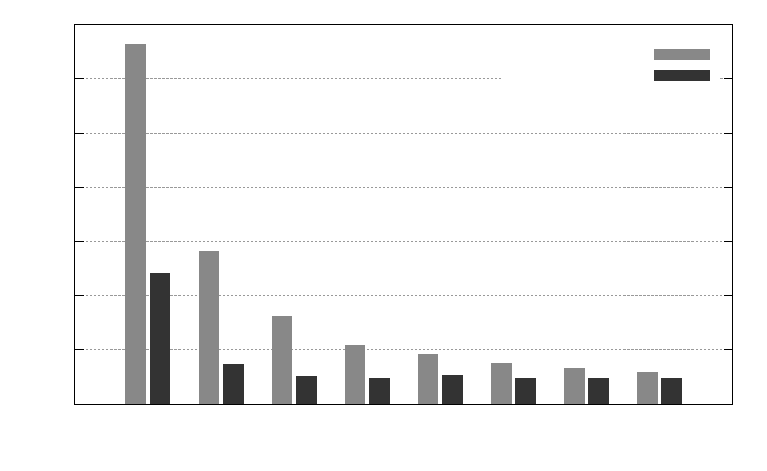
\includegraphics{../data/performance/plots/cores/helios-plot}}%
    \gplfronttext
  \end{picture}%
\endgroup

  \vspace{.5\baselineskip}
  \caption[Einfluss der zur Verfügung stehenden Rechenkerne auf durchschnittliche Laufzeit der Typüberprüfung von Flow und TypeScript]{
    Einfluss der zur Verfügung stehenden Rechenkerne auf durchschnittliche Laufzeit der Typüberprüfung von Flow 0.96 und TypeScript 3.5 der Projekte Components und Helios.
  }

  \vspace{\baselineskip}
  \caption*{
    \small
    Gemessen mit Intel Core i7-6700 CPU mit 3,4~GHz (System D).
  }

  \label{fig:plot-cores}
\end{figure}

Sowohl bei Flow, als auch bei TypeScript wird die Laufzeit der Berechnung bereits bei Verwendung von zwei Rechenkernen im Vergleich zu einem einzigen Kern deutlich verringert. Obwohl TypeScript eine parallelisierte Kompilierung grundsätzlich nicht unterstützt, wird auch dieser Prozess beschleunigt, weil der TypeScript-Compiler durch Node.js ausgeführt wird und diese Umgebung standardmäßig mehrere Threads startet, um beispielsweise teure Ein- und Ausgabeoperationen auf weitere Prozessorkerne auszulagern~\autocite{NODE:THREADS}. Für mehr als drei Kerne bleibt die Laufzeit von TypeScript daraufhin in beiden Projekten aber in etwa konstant. Wie die Messwerte und Diagramme zeigen, verringert sich die Laufzeit von Flow dagegen mit wachsender Zahl zur Verfügung stehender Rechenkerne aufgrund der Unterstützung von Multithreading stetig. Ab etwa fünf Kernen sind die Zugewinne allerdings nur noch gering, was auf den zunehmend größeren Overhead durch die notwendige Synchronisierung der Threads zurückgeführt werden könnte. Bei maximal möglicher Parallelisierung durch acht Kerne, erreicht Flow bei Helios nahezu die Laufzeit von TypeScript.

\subsubsection{Fazit}

Die angestrebte Verbesserung der Performance durch die Migration zu TypeScript kann im vorliegenden Fall nur als teilweise erreicht betrachtet werden, da nur in drei Fällen bei Helios tatsächlich geringere Laufzeiten für eine vollständige Typüberprüfung gemessen wurden. Die stark parallelisierte Architektur von Flow scheint der von TypeScript bezüglich der Geschwindigkeit in den meisten Fällen überlegen. Es wird aber vermutet, dass die Performance von TypeScript gesteigert werden könnte, wenn auch hier die Berechnung der Typkorrektheit nebenläufig wäre. Laut Aussage eines Entwicklers von TypeScript im März 2019 wird die Implementierung von Multithreading im TypeScript-Compiler bereits in Betracht gezogen~\autocite{TS:MULTICORE}.

\subsection{Zukunftssicherheit und Transparenz der Technologie}

Das letzte Ziel der Migration zu TypeScript war schließlich die Zukunftssicherheit zu steigern, da angenommen wird, dass die Entwicklung von TypeScript transparenter abläuft als bei Flow. Hierzu wurden in Abschnitt~\ref{sec:goal:transparency} verschiedene Fragestellungen aufgeworfen, die im Folgenden beantwortet werden sollen.
Die erste Frage betrifft die Verfügbarkeit eines öffentlich einsehbaren Projektplans (\textit{Roadmap}) in welchem strategische Entscheidungen kommuniziert werden, sodass die langfristige Weiterentwicklung der Technologie besser eingeschätzt werden kann. Für Flow existiert derzeit keine solche Roadmap: Eine entsprechende Anfrage im November 2017 auf GitHub blieb durch das Entwicklerteam von Flow unbeantwortet~\autocite{FLOW:GITHUB:ROADMAP}. Ein Mitarbeiter von Facebook bestätigte aber im Januar 2019, dass beabsichtigt werde zukünftig einen Projektplan für Flow zu veröffentlichen~\autocite{FLOW:GITHUB:ROADMAP_FUTURE}. Die Entwicklung von TypeScript ist an dieser Stelle deutlich transparenter: So werden auf GitHub einerseits perspektivische Ziele der Programmiersprache kommuniziert, andererseits konkrete Halbjahrespläne ausführlich dargelegt~\autocite{TS:ROADMAP}. Benutzer von TypeScript können damit sehr gut beurteilen, welche Funktionen in Zukunft zu erwarten sind und wie diese priorisiert werden.

Sowohl Flow, als auch TypeScript werden quelloffen auf der Plattform GitHub entwickelt, sodass Benutzer die Möglichkeit haben Probleme (\textit{Issues}) zu melden und sich in die Weiterentwicklung der Systeme einzubringen. Um zu untersuchen wie schnell derartige Tickets bearbeitet werden, wurden für Flow und TypeScript entsprechende Daten durch die Programmierschnittstelle\footnote{Application Programming Interface (API).} von GitHub~\autocite{GITHUB:API} erhoben. Anhand von 3,8 bzw. 20 Tausend Einträgen von Flow und TypeScript wurde ermittelt wie viel Zeit im Median zwischen der Erstellung und der Behebung eines Problemberichts vergeht: Hierbei ergibt sich für Flow bzw. TypeScript ein Wert von 11,58 bzw. 6,61 Tagen. Zwar muss das Schließen eines Tickets nicht in jedem Fall bedeuten, dass tatsächlich ein Programmfehler vorlag und dieser korrigiert wurde, dennoch kann bei TypeScript somit insgesamt eine schnellere Bearbeitung von gemeldeten Problemen festgestellt werden.

Die letzte Fragestellung aus Kapitel~\ref{chap:analysis} betrifft die Zukunftssicherheit von Flow bzw. TypeScript, also ob die langfristige Unterstützung der Systeme durch die Autoren Facebook bzw. Microsoft gewährleistet ist. Weil keine Roadmap für Flow vorliegt und bekannt wurde, dass selbst interne Projekte bei Facebook wie zum Beispiel \textit{Jest}~\autocite{SOFTWARE:JEST} zu TypeScript migrieren~\autocite{JEST_TS}, bestand bei einigen Entwicklern Verunsicherung darüber, ob Facebook die Fortentwicklung des Systems weiterhin fokussiert. Diese Zweifel wurden jedoch von einem der Autoren von Flow Avik Chaudhuri im bereits erwähnten Artikel \enquote{\citetitle{FLOW:UPDATE_2019}}~\autocite{FLOW:UPDATE_2019} ausgeräumt. Er betont, dass Facebook intern nach wie vor primär Flow einsetze und die Zukunft des Systems gesichert sei. Im Fall von TypeScript besteht wie ausgeführt eine öffentlich einsehbarer Projektplan, sodass von einer fortwährenden Unterstützung durch Microsoft ausgegangen werden kann.

Zusammenfassend kann gesagt werden, dass die Migration zu TypeScript tatsächlich Vorteile bezüglich der Zukunftssicherheit und Transparenz bietet. Im Vergleich zu Flow besteht hier eine deutlich höhere Planungssicherheit bezüglich der Weiterentwicklung des Typsystems, weil bei TypeScript eine Roadmap öffentlich zugänglich ist. Auch Fehlerberichte auf GitHub werden bei TypeScript insgesamt schneller bearbeitet. Die langfristige Unterstützung der Systeme durch die ursprünglichen Autoren ist in beiden Fällen anzunehmen.

\section{Erfüllung der technischen Anforderungen}

Nachdem die Erfüllung der Zielvorgaben durch den Wechsel zu TypeScript diskutiert wurden, soll im Folgenden auch die Einhaltung der technischen Anforderungen an den Flow-Transpiler untersucht werden.

\subsection{Äquivalente und vollständige Übersetzung der Flow-Typen}
\label{sec:interpretation:equivalent-translation}

\subsubsection{Äquivalenz der Übersetzungen}

Als erste und wichtigste technische Anforderung an den Transpiler wurde die äquivalente und vollständige Übersetzung der gesamten Flow-Syntax nach TypeScript definiert. Die äquivalenten TypeScript-Ausdrücke der verschiedenen Flow-Typen konnten dabei mehrheitlich einfach gefunden werden, weil TypeScript einen sehr ähnlichen Funktionsumfang wie Flow besitzt und sich oftmals nur die Schlüsselwörter unterscheiden\footnote{Vgl. Übersetzungstabellen in Abschnitt~\ref{sec:flow-transpilation}.}. Kompliziertere, nicht offensichtliche Transformationen wurden experimentell bestimmt.

\begin{lstlisting}[
  label={code:transpiler-warnings},
  caption={Ausgabe von Warnungen bei Autreten nicht äquivalent übersetzbarer Flow-Typen.},
  emph={Warning},
]
Transpiling example.js...

  1 | // @flow
> 2 | const existentialType: * = String(2 * 3);
    |                       ^
  Warning: Flow's Existential Type (*) is not expressible in TypeScript.
           It will be replaced with 'any'.
           See https://github.com/Microsoft/TypeScript/issues/14466.
\end{lstlisting}

Für einige, wenige Typen existiert keine absolut bedeutungsgleiche Übersetzung, weil TypeScript manche der Funktionen von Flow nicht unterstützt. Infolgedessen kommt es hier bei der Transpilierung zwingend zu einem Verlust von Typinformation, was in neuen Typfehlern resultieren kann. Die inkorrekte Transformation derartiger Typen wird gemäß Anforderung~\ref{sec:requirement:completeness} akzeptiert, jedoch muss der Benutzer bei Auftreten eines solchen Falls gewarnt werden. Quelltext~\ref{code:transpiler-warnings} zeigt wie eine solche Warnung aufgebaut ist. Dabei wird einerseits die genaue Position des verursachenden Flow-Typs im Quelltext angegeben, andererseits wird der Benutzer über die Hintergründe der Warnung durch einen Link informiert. Nachfolgend wird dargelegt, welche der Funktionen von Flow nicht absolut korrekt übersetzt werden können und wie dies jeweils innerhalb des Transpilers gehandhabt wird.

\begin{itemize}
  \item {\libertineSB{Existential type}}\\*
    In TypeScript existiert kein Typ, der Flows \type{Existential type} entspricht~\autocite{TS:GITHUB:NO_EXISTENTIAL_TYPE}. Wie Quelltext~\ref{code:transpiler-warnings} bereits andeutet, wird dieser Typs deswegen durch den Typ \type{any} ersetzt. Weil \type{any} Supertyp jeden Typs ist, geht damit Typinformation verloren, sofern Flow zuvor einen konkreteren Typ inferieren konnte. Jedoch gibt die Dokumentation von Flow an, dass dies oftmals nicht funktioniert und der \type{Existential type} deshalb in diesen Fällen tatsächlich äquivalent zu \type{any} ist~\autocite{FLOW:LINT_RULE_REFERENCE}.
  \medbreak
  \item {\libertineSB{Index-Signaturen in Objekttypen}}\\*
    Durch eckige Klammern kann in Objekttypen ein Index, also die Abbildung eines Typs von Namen auf Werte eines anderen Typs, angegeben werden\footnote{Vgl. Tabelle~\ref{tab:flow-base-types}.}. Flow unterstützt hierbei jeden beliebigen Typ für die Attributnamen, TypeScript hingegen nur \code{string} und \code{number}~\autocite{TS:HANDBOOK:INTERFACES}. Infolgedessen entfernt der Transpiler Index-Signaturen, die von diesen zugelassenen Typen abweichen, und fügt stattdessen jeweils eine Signatur für \code{string} und \code{number} ein, um die größtmögliche Menge von Schlüsseltypen zu erlauben.
  \medbreak
  \item {\libertineSB{Opaque type}}\\*
    Auch opake Typen werden durch TypeScript nicht unterstützt~\autocite{TS:GITHUB:NO_OPAQUE_TYPE}. Deshalb wird dieser Typ bei der Übersetzung durch ein Typalias ersetzt, das auf den gleichen Typ verweist.
  \medbreak
  \item {\libertineSB{Rückgabewert von Konstruktoren}}\\*
    Flow ermöglicht es den Rückgabewert von Konstruktorfunktionen explizit anzugeben. Dies ist in TypeScript bewusst verboten, weil es im Allgemeinen als schlechter Programmierstil gilt, wenn ein Konstruktor etwas anderes als eine Klasseninstanz zurückliefert~\autocite{TS:GITHUB:CONSTRUCTOR_RETURN_TYPE}. Ein solcher Rückgabewert wird deswegen durch den Transpiler entfernt, damit keine fehlerhafte TypeScript-Syntax entsteht.
  \medbreak
  \item {\libertineSB{Varianz}}\\*
    Ein letzter Aspekt von Flow, der in TypeScript in einigen Fällen nicht abbildbar ist, ist die Varianz von Typen. Weil die Syntax von TypeScript nur Kovarianz (Schlüsselwort \code{readonly}) unterstützt, werden die Varianz-Signaturen von Flow für alle anderen Fälle verworfen. Dies beinhaltet neben Objektattributen beispielsweise auch Typparameter, die in Flow entsprechend annotiert werden können.
\end{itemize}

Neben diesen Flow-Funktionen, die prinzipiell nicht bedeutungsgleich übersetzt werden können, konnte darüber hinaus für die drei Hilfstypen \type{Object map}, \type{Object map with key} und \type{Tuple map} wie ausgeführt kein TypeScript-Ausdruck gefunden werden, der diesen entspricht. Deshalb ist die äquivalente Transformation der Typisierung auch in diesen drei Fällen nicht gegeben, weil diese Typen durch \type{any} ersetzt werden.

\subsubsection{Vollständigkeit der Transformationen}

Wie bereits in Abschnitt~\ref{sec:requirement:completeness} dargelegt ist der vollständige Funktionsumfang der Implementierung durch die Spezifikation des Parsers~\autocite{BABEL:PARSER_SPEC} von Babel präzise definiert, weil das Dokument festlegt, welche Knoten des abstrakten Syntaxbaums Flow-Syntax darstellen. Sofern sämtliche dieser Elemente korrekt in ihr TypeScript-Gegenstück transformiert werden, so ist die Vollständigkeit erreicht. Dies setzt vorraus, dass der abstrakte Syntaxbaum von Babel tatsächlich jegliche Flow-Syntax abbildet. Es konnte kein Beleg dafür gefunden werden, dass diese Annahme falsch ist.

Ein weiterer Aspekt, der zur Erzielung einer vollständigen Umsetzung beiträgt, ist die Typisierung von Babel, da diese zum Beispiel den Vereinigungstyp \code{Flow} bereitstellt, der alle Knotentypen von Flow umfasst~\autocite{BABEL:TYPES}. Somit kann durch eine geeignete Typisierung statisch überprüft werden, ob das Programm alle Elemente eines solchen Vereinigungstyps verarbeitet. Auch hier muss die Vorraussetzung gelten, dass die Typisierung von Babel bezüglich Flow korrekt ist.
Der umgesetzte Transpiler verwendet diesen Ansatz beispielsweise innerhalb der zentralen Umwandlungsfunktion für beliebige Flow-Typen (\code{convertFlowType}\footnote{Vgl. Quelltext~\ref{code:convert-flow-type}.}), sodass statisch garantiert werden kann, dass dabei ausnahmslos alle Elemente des Vereinigungstyps \code{FlowType} transformiert werden.

Die Erzielung der Korrektheit und Vollständigkeit der Transformationen wird durch den in Abschnitt~\ref{sec:tdd} dargelegten Ansatz der testgetriebenen Entwicklung gewährleistet. In der Dokumentation von Flow~\autocite{FLOW:TYPE_ANNOTATIONS} wird die Syntax aller Sprachkonstrukte beschrieben, sodass bekannt ist, welche Typen prinzipiell möglich sind. Durch Anlegen von Fixture-Dateien kann damit die korrekte Übersetzung sämtlicher Flow-Funktionen umfangreich getestet werden. Wie ausgeführt sind insgesamt \numberOfTests Testfälle entstanden, um alle Basis- und Hilfstypen sowie Typdeklarationen zu überprüfen. Durch eine hohe Testabdeckung von 93\% wird darüber hinaus sichergestellt, dass die verschiedenen Programmverzweigungen des Transpilers tatsächlich die angestrebte Funktionalität umsetzen.

\subsubsection{Vergleich mit Ansätzen von Kikura und Barabash}

Die zwei betrachteten Aspekte der Äquivalenz und Vollständigkeit der Transformationen sollen auch für die Ansätze von Kikura und Barabash beleuchtet werden, um das erzielte Ergebnis einzuordnen. Dabei wird untersucht, ob diese Plugins bei Anwendung auf die angelegten Fixture-Tests zur Erprobung der korrekten Übersetzung der Flow-Typisierung zu den gleichen Ergebnissen kommen.
Tabelle~\ref{tab:correctness-comparison} auf Seite~\pageref{tab:correctness-comparison} zeigt bei welchen Testfälle hierbei eindeutig eine fehlerhafte Transformation vorgenommen wird. Darunter wird einerseits die semantisch inkorrekte Übersetzung eines Typs, andererseits unzulässige TypeScript-Syntax in der Ausgabe verstanden. Eine solche invalide Syntax entsteht beispielsweise dann, wenn Spezialfälle nicht richtig behandelt werden. Weil sich die Tabelle am Aufbau der Fixture-Tests orientiert, werden nicht alle einzelnen Typen wie in Kapitel~\ref{chap:basics} separat, sondern gruppiert, aufgelistet. Die Kategorie \enquote{\textit{Primitives}} enthält dabei zum Beispiel die Tests für alle primitiven Flow-Typen wie \type{Number type}, \type{String literal type} et cetera.

\medbreak
\begin{table}[p]
  \caption{Fehlerhafte Übersetzung von Flow-Typen bei Kikura~\autocite{KIKURA:FLOW_TO_TS} und Barabash~\autocite{BARABASH:FLOW_TO_TS} im Vergleich zur vorliegenden Implementierung (\Lightning~=~Programmabsturz).}
  \footnotesize
  \begin{tabu} to \textwidth {@{}lr|rr|rr|rX@{}}
    \midrule
    \multicolumn{2}{l|}{} & \multicolumn{2}{l|}{\large\textsc{kikura}} & \multicolumn{2}{l|}{\large\textsc{barabash}} &  \multicolumn{2}{l}{\large\textsc{vorl. impl.}} \\
    \rowfont[l]{\libertineSB} Typ & Testfälle & Fehler & rel. Anteil & Fehler & rel. Anteil & Fehler & {} \\
    \midrule
    Any type              &   8 & 0          & 0      &  0         & 0        & 0 & {} \\
    Array type            &  13 & 0          & 0      &  2         & 15,5\%   & 0 & {} \\
    Class type            &  43 & \Lightning & --     &  4         &  9,3\%   & 0 & {} \\
    Empty type            &   7 & \Lightning & --     &  0         & 0        & 0 & {} \\
    Function type         &  34 & \Lightning & --     &  4         & 11,8\%   & 0 & {} \\
    Generics              &  17 & \Lightning & --     &  1         &  5,9\%   & 0 & {} \\
    Interface type        &  61 & \Lightning & --     & \Lightning & --       & 0 & {} \\
    Intersection type     &  29 & \Lightning & --     &  2         &  6,9\%   & 0 & {} \\
    Maybe type            &  27 & \Lightning & --     & 23         & 85,2\%   & 0 & {} \\
    Mixed type            &   6 & 0          & 0      &  0         & 0        & 0 & {} \\
    Module type           &  32 & \Lightning & --     &  6         & 18,8\%   & 0 & {} \\
    Object type           & 122 & \Lightning & --     & \Lightning & --       & 0 & {} \\
    Opaque type           &  10 & 2          & 20,0\% &  6         & 60,0\%   & 0 & {} \\
    Primitives            &   9 & 0          & 0      &  0         & 0        & 0 & {} \\
    This type             &   8 & 0          & 0      & \Lightning & --       & 0 & {} \\
    Tuple type            &   5 & 0          & 0      &  1         & 20,0\%   & 0 & {} \\
    Type alias            &  22 & \Lightning & --     &  3         & 13,6\%   & 0 & {} \\
    Type cast             &  16 & 0          & 0      &  0         & 0        & 0 & {} \\
    Type declarations     &  44 & \Lightning & --     & 14         & 31,8\%   & 0 & {} \\
    Typeof type           &  20 & 3          & 15,0\% &  2         & 10,0\%   & 0 & {} \\
    Union type            &  19 & \Lightning & --     &  1         &  5,3\%   & 0 & {} \\
    Call                  &   6 & \Lightning & --     &  0         & 0        & 0 & {} \\
    Difference            &  11 & 0          & 0      &  0         & 0        & 0 & {} \\
    Element type          &  13 & 0          & 0      &  0         & 0        & 0 & {} \\
    Exact                 &   7 & 0          & 0      &  1         & 14,3\%   & 0 & {} \\
    Existential type      &   5 & 0          & 0      &  0         & 0        & 0 & {} \\
    Keys                  &   5 & 0          & 0      &  0         & 0        & 0 & {} \\
    None maybe type       &   6 & 4          & 66,7\% &  0         & 0        & 0 & {} \\
    Property type         &   8 & 0          & 0      &  0         & 0        & 0 & {} \\
    Rest                  &  13 & \Lightning & --     &  0         & 0        & 0 & {} \\
    Shape                 &  11 & 3          & 22,3\% &  0         & 0        & 0 & {} \\
    \libertineSB{Insgesamt} & \libertineSB{637} & \libertineSB{12} & \libertineSB{1,9\%} & \libertineSB{70} & \libertineSB{11,0\%} & \libertineSB{0} & {} \\
    \midrule
    \label{tab:correctness-comparison}
  \end{tabu}
\end{table}


Die Übersetzung der Flow-Typen durch Kikura ist in 98,1\% der Fälle korrekt. Jedoch können dabei nur 17 der 31 Testfälle überhaupt betrachtet werden, weil die Transpilierung der verbleibenden 14 Eingabedateien gänzlich fehlschlägt, da hier jeweils Laufzeitfehler auftreten (Symbol~\Lightning). Somit ist nicht nachvollziehbar, ob eventuell weitere Fehler vorliegen. Auch bei Barabash stürzt das Programm bei drei der Fixture-Dateien ab, sodass diese Tests nicht bewertet werden können. In 89,0\% der anderen Fälle wird die Transformation hier aber korrekt umgesetzt. Die Gründe, warum die Übersetzungen bei Kikura und Barabash in einigen Fällen falsch sind, sind vielfältig. Im Folgenden werden einige der Ursachen aufgelistet:

\begin{itemize}
  \item Wie ausgeführt dürfen Konstruktoren in TypeScript keine Rückgabewerte deklarieren. Sofern diese, wie hier bei Barabash, nicht entfernt werden, so entsteht ein Syntaxfehler.
  \item Flow erlaubt es Funktionsparameter, die mit einem Standardwert~\autocite{MDN:DEFAULT_PARAMS} initialisiert werden, als optional zu markieren\footnote{Zum Beispiel: \code{function f(optional?: number = 10) \{\}}.}. Derartige Parameter dürfen in TypeScript nicht optional sein, sodass die Notation durch den Transpiler entsprechend angepasst werden muss.
  \item Bei Barabash wird der \type{Nullable type} (\type{Maybe type}) falsch übersetzt. Statt der Vereinigung aus dem angegeben Typ, \code{null} und \code{undefined} wird hier der Typ lediglich mit \code{null} kombiniert.
  \item Kikura wandelt opake Typen wie die vorliegende Umsetzung in reguläre Typaliase um. Jedoch werden dabei bestehende Typparameter verworfen.
  \item Schließlich werden bei beiden Ansätzen einige der Hilfstypen überhaupt nicht transformiert und einfach in die Ausgabe übernommen. Weil diese Typen in TypeScript undefiniert sind, entsteht auch so ein Fehler.
\end{itemize}

Insgesamt treten bei Kikura zwar weniger fehlerhafte Transformationen als bei Barabash auf, aber das Plugin stürzt auch bei fast der Hälfte der Eingabedateien ab, was darauf hindeutet, dass noch viele Spezialfälle außer Acht gelassen wurden. Der Ansatz von Barabash ist hier bedeutend stabiler, jedoch wurden in Summe mehr Fehler aufgedeckt. Da hier allerdings auch deutlich mehr Testfälle untersucht werden konnten (161 bei Kikura versus 466 bei Barabash), ist dies zu erwarten. Zusammenfassend lässt sich sagen, dass beide Ansätze offenbar viele Grenzfälle der Übersetzung derzeit noch nicht korrekt behandeln, sodass verschiedene semantische und syntaktische Probleme in der Ausgabe entstehen.

\subsubsection{Fazit}

Durch die Fixture-Tests können sowohl die Korrektheit, als auch die Vollständigkeit der Übersetzung der Flow-Typen nach TypeScript überprüft werden. Jedoch setzt dies voraus, dass die Testfälle tatsächlich einen Großteil der möglichen Typisierung durch Flow abbilden. Obwohl die Tests mit großer Sorgfalt angelegt wurden, kann nicht ausgeschlossen werden, dass gewisse Fälle nicht bedacht wurden. In Anbetracht dessen, dass die Testfälle aber bei den zum Vergleich herangezogenen Ansätzen von Kikura und Barabash noch viele Schwachstellen offen gelegt haben, kann angenommen werden, dass diese zumindest den wesentlichen Teil der Szenarien abdecken. Auch die erfolgreiche praktische Anwendung des umgesetzten Transpilers auf die Projekte von TeamShirts deutet stark darauf hin, dass sowohl die Semantik als auch die Syntax der Flow-Typen korrekt nach TypeScript überführt wird. Die Äquivalenz der Transformationen ist dabei wie beschrieben nur in einzelnen Fälle nicht gegeben.

\subsection{Semantisch äquivalente Transpilierung des Quelltexts}

Eine weitere wichtige Anforderung an den Transpiler ist, dass die Semantik des ursprünglichen JavaScript-Programms durch die Übersetzung nicht verändert werden darf, damit keine neuen Programmfehler in den Quelltext eingeschleust werden. Die korrekte Übersetzung der Semantik der Flow-Typen wurde bereits im vorherigen Abschnitt behandelt. Hierbei ist anzumerken, dass die statische Typisierung aber ohnehin keinen Einfluss auf die Semantik des Programms zur \emph{Laufzeit} hat, weil die Typen vor der Auslieferung vollständig entfernt werden. Dies setzt vorraus, dass die Programm-Transformation tatsächlich nur die Typisierung adressiert und keine unbeabsichtigte Nebenwirkung, wie zum Beispiel das Einfügen neuer Anweisungen in das Programm, hat. Ein weiterer Aspekt des umgesetzten Transcompilers, der zu abweichender Semantik führen könnte sind die in Abschnitt~\ref{sec:optimizations} beschriebenen optionalen Optimierungen der Ausgabe. Durch die Option \enquote{\code{replace-decorators}} werden beispielsweise Dekoratoren in bedeutungsgleiche verschachtelte Funktionsaufrufe umgewandelt. Die Einhaltung dieser Einschränkungen wird wie ausgeführt durch die Fixture-Tests überprüft.

% TODO: check numbers about coverage
Ein formaler Beweis der semantischen Äquivalenz ist aufgrund des Umfangs der zwei migrierten Projekte nicht durchführbar. Jedoch kann durch Betrachtung der bestehenden Modultests die Beibehaltung der Programmwirkung nach der Übersetzung zumindest approximativ verifiziert werden. Kritisch anzumerken ist, dass dieser Ansatz nur bei einer entsprechend hohen Testabdeckung aussagekräftig ist. Während diese bei Components bei 90,5\% liegt, wird bei Helios nur ein Anteil von 18,0\% erreicht.
Nachdem alle nicht-strikten Typfehler in beiden Projekten korrigiert worden sind, wurden die Modultests beider Projekte ausgeführt. Keiner der 373 Tests von Components und 326 Tests von Helios schlug dabei fehl, sodass die semantisch korrekten Überführung des ursprünglichen Quelltexts nach TypeScript zumindest für das Projekt Components wahrscheinlich ist. Bei der praktischen Erprobung der zwei Projekte wurde allerdings in vier Fällen ein fehlerhaftes Verhalten der Webanwendung festgestellt. Jedoch konnte jedes dieser Probleme auf eine fehlerhafte händische Korrektur neuer Typfehler zurückgeführt werden. Es wird somit angenommen, dass der Transpiler die Semantik durch die Übersetzung tatsächlich beibehält und nur wo nötig, zum Beispiel bei nicht unterstützten Flow-Typen, modifiziert.

\subsection{Unterstützung aktueller und vorläufiger JavaScript- sowie JSX-Syntax}

Die Anforderung aktuelle und vorläufige JavaScript- sowie JSX-Syntax zu unterstützen war eines der grundlegenden Kriterien, anhand derer in Abschnitt~\ref{sec:js-transpilers} verschiedene Parser, Codegeneratoren und Transpiler bezüglich ihrer Eignung als Basis für die Umsetzung des Flow-Transpilers verglichen wurden. Wie dort bereits ausgeführt ist Babel nach Kenntnisstand des Autors das einzige Werkzeug, dass sowohl jegliche aktuelle, als auch vorläufige JavaScript-Syntax einlesen und verarbeiten kann. Deshalb wurde der umgesetzte Transpiler auf Basis von Babel implementiert, um diese Anforderung zu erfüllen. Wie die erfolgreich durchgeführte Transpilierung der zwei Projekte von TeamShirts beweist, ist die Verarbeitung derartiger Syntax tatsächlich möglich.

Auch hier sollen die Ansätz von Kikura und Barabash bezüglich dieser Anforderung untersucht werden, um die Ergebnisse zu vergleichen. Beide Projekte wurden wie die vorliegende Implementierung als Babel-Plugin umgesetzt, sodass aktuelle ECMAScript-Syntax vollständig unterstützt wird. Darüber hinaus ermöglichen beide Projekten die Verarbeitung von JSX-Syntax und der vorläufigen Erweiterungen \textit{Class field declarations for JavaScript}~\autocite{ES_PROPOSAL:CLASS_FIELDS} und \textit{Dynamic imports}~\autocite{ES_PROPOSAL:DYNAMIC_IMPORTS}. Klassendekoratoren werden jedoch von keinem der Ansätzen unterstützt, weshalb Dateien, die derartige Syntax verwenden, nicht transpiliert werden können. Darüber hinaus wurde festgestellt, dass bestimmte korrekte Flow-Syntax in Objekttypen bei Barabash zu Laufzeitfehlern führt, weil offenbar in diesen Fällen Knoten des abstrakten Syntaxbaums fehlerhaft transformiert werden\footnote{Vgl. Tabelle~\ref{tab:correctness-comparison}}. Auch bei Kikura treten bei Verwendung mancher Flow"=Notationen wie zum Beispiel bei der expliziten Typumwandlung vereinzelt Syntaxfehler auf. Die vollständige Verarbeitung der Codebasis der zwei Projekte von TeamShirts wäre somit mit den Ansätzen von Kikura und Barabash nicht möglich.

\subsection{Verarbeitung gesamter Projektverzeichnisse}

Wie in Abschnitt~\ref{sec:cli-program} bereits ausführlich dargelegt, wurde der Transpiler um ein Kommandozeilenprogramm erweitert, um die Anforderung der Verarbeitung gesamter Verzeichnisse zu realisieren. Die Anwendung erwartet dabei eine oder mehrere Dateien bzw. Verzeichnisse als Argument und setzt daraufhin die Übersetzung dieser Eingaben mit Hilfe des Babel-Plugins um.
Durch die interne Verwendung der Bibliothek \textit{Glob}~\autocite{NPM:GLOB} können hierbei beliebig komplexe Wildcard-Muster (\textit{glob patterns}) verarbeitet werden, um bestimmte Datei- oder Verzeichnistypen ein- und auszuschließen. Die Glob-Notation ähnelt regulären Ausdrücken in einigen Aspekten konzeptionell, sodass auch die Angabe komplizierterer Muster, wie beispielsweise die Negation von Ausdrücken oder die Angabe einer Gruppe von alternativen Werten, möglich ist~\autocite{MAN:GLOB}.
Die in Abschnitt~\ref{sec:requirement:batch-processing} definierten Anforderungen, dass einerseits Verzeichnisse rekursiv verarbeitet werden, andererseits die Menge der zu übersetzenden Dateien flexibel eingegrenzt werden können muss, wurden somit erfüllt.

Von den zwei zum Vergleich betrachteten Ansätzen, ermöglicht lediglich der Flow-Transpiler von Barabash die Übersetzung ganzer Projektverzeichnisse durch ein integriertes Kommandozeilenprogramm~\autocite{BARABASH:FLOW_TO_TS}. Das Babel-Plugin von Kikura bietet eine solche Funktionalität nicht.

\subsection{Beibehaltung der Quelltext-Formatierung}
\label{sec:results-formatting}

\subsubsection{Ergebnisse}

Die letzte technische Anforderung an den Transpiler ist die möglichst originalgetreue Formatierung der Ausgabe. Weil diese bei Verwendung des Babel-Codegenerators aus den dargelegten Gründen nicht ohne Weiteres umsetzbar ist, wurde eine Formatierungsroutine auf Basis des Werkzeugs Prettier~\autocite{SOFTWARE:PRETTIER} implementiert. Mittels händischer Überprüfung des erzeugten TypeScript-Codes der zwei Projekte von TeamShirts, wurden inkorrekt formatierte Dateien ermittelt. Hierunter werden Dateien verstanden in denen Ausdrücke, mit Ausnahme von Objektliteralen, anders als im ursprünglichen Quelltext umgebrochen oder Leerzeilen und Kommentare falsch platziert werden. Sobald eines dieser Kriterien vorliegt, wird die Formatierung als fehlerhaft betrachtet.

Tabelle~\ref{tab:results-formatting} zeigt die Ergebnisse dieser manuellen Überprüfung. Dabei werden die erreichten Werte der vorliegende Implementierung (\textit{Reflow}) dem Ansatz von Barabash~\autocite{BARABASH:FLOW_TO_TS} gegenüber gestellt, um die Zahlen besser einordnen zu können. Das Babel-Plugin von Kikura~\autocite{KIKURA:FLOW_TO_TS} bietet keine Möglichkeit die Ausgabe zu formatieren und wird daher nicht in den Vergleich miteinbezogen.
Wie die Tabelle zeigt, schlägt das Verfahren sowohl in der vorliegenden Umsetzung, als auch bei Barabash in einigen Fällen fehl. Jedoch erzielt die in dieser Arbeit implementierte Formatierungsroutine insgesamt bessere Ergebnisse: Während hier in Summe 32 Dateien~(4,7\%) fehlerhaft formatiert werden, liegt der Anteil bei Barabash bei 48 Dateien~(7,0\%).

\medbreak
\begin{table}[tbh]
  \footnotesize
  \begin{tabu} to \textwidth {@{}lrrrrrr@{}}
    \midrule
    \libertineSB{Projekt} & \libertineSB{Dateien} & \libertineSB{falsch formatiert} & \libertineSB{rel. Anteil} & \libertineSB{Zeilen~$+$} & \libertineSB{Zeilen~$-$} & \libertineSB{Zeilen insg.} \\
    \midrule
    Components & 331 & 11 & 3,32\% & 2.564 & 2.417 & 32.240 \\
    Helios     & 353 & 21 & 5,95\% & 4.604 & 3.873 & 45.436 \\
    \midrule
    insgesamt  & 684 & 32 & 4,68\% & 7.168 & 6.290 & 77.675 \\
    \midrule
  \end{tabu}
  \caption{Ergebnisse der Formatierung der Ausgabequelltexte.}
  \label{tab:results-formatting}
\end{table}


\subsubsection{Fehleranalyse}

Zur Feststellung der Ursachen der fehlerhaften Formatierung durch den in dieser Arbeit umgesetzten Transpiler, wurde die Verarbeitung der inkorrekt ausgegebenen Dateien untersucht. Weil das Verfahren zeilenbasiert arbeitet, ist die Konsistenz der Umbrüche für das Gelingen der Formatierung entscheidend, da es andernfalls zu einem Versatz der betrachteten Eingabe- und Ausgabgezeilen kommt. Die Betrachtung der Originaldateien, welche fehlerhaft formatiert wurden, hat gezeigt, dass dies in Folge von bestimmten, eher selten vorkommenden Quelltext-Formatierung auftritt. Nachfolgend soll das Problem anhand eines Beispiel für einen solchen Fall veranschaulicht werden:

\begin{lstlisting}[
  label={code:wrong-formatting:flow},
  caption={Beispiel für Formatierung des Original-Quelltexts, die falsch in die Ausgabe übernommen wird.}
]
if (
  a &&
  b &&    // Kommentar, der Zweck von 'b' beschreibt
  c === 0 // Kommentar, der Zweck von 'c' beschreibt
) {
  // ...
}
\end{lstlisting}

Der boolesche Ausdruck, der als Argument der bedingten Anweisung in Zeile~1 dient, wird mehrmals umgebrochen, damit der Zweck der einzelnen Elemente durch einen Zeilenkommentar erläutert werden kann. Der umgesetzte Flow-Transpiler ignoriert Kommentare der Eingabe bei Generierung der TypeScript-Ausgabe generell, weil Babel diese wie ausgeführt ohnehin zum Teil falsch platziert. Erst durch die Formatierungsroutine werden die Kommentare im Nachgang wieder eingefügt, um deren korrekte Positionierung zu erzielen. Diese schlägt für das Beispiel fehl, weil der boolesche Ausdruck in der erzeugten Ausgabe aufgrund der entfernten Kommentare nicht länger umgebrochen wird (vgl. Quelltext~\ref{code:wrong-formatting:ts}). Da der Zeilenumbruch in der Ein- und Ausgabe in diesem Fall somit inkonsistent ist, schlägt die Übertragung der Formatierung beim Vergleich dieser und aller nachfolgenden Zeilen fehl.

\begin{lstlisting}[
  % float,
  % floatplacement=H,
  label={code:wrong-formatting:ts},
  caption={Generierte TypeScript-Ausgabe der Eingabe in~\ref{code:wrong-formatting:flow} \emph{vor} Ausführung der Formatierungsroutine.}
]
if (foo && bar && baz === 0) {
  // ...
}
\end{lstlisting}

Wie die weitere Fehleranalyse gezeigt hat, ergibt sich bei der Auflistung der formalen Parameter von Funktionen die gleiche Problematik, wenn diese analog zum Beispiel umgebrochen werden. Zur Lösung dieser fehlerhaften Fälle, sollte die angepasste Version von Prettier so erweitert werden, dass auch das Argument bedingter Anweisungen und die Auflistung  von Parametern stets umgebrochen werden.

\subsubsection{Fazit}

Zwar konnte die Anforderung nicht vollständig umgesetzt werden, weil nicht alle Ausgabedateien korrekt formatiert werden, dennoch wurde der Programmierstil in 95,3\% der Fälle akkurat beibehalten. Da die manuelle Korrektur der insgesamt 32 fehlerhaften Dateien mit geringem Zeitaufwand durchführbar ist, kann die geforderte Funktion damit als größtenteils erfüllt betrachtet werden.
